\chapter{La méthode des éléments finis}\label{Ch-MEF}
\begin{abstract}
Une fois le travail précédent accompli, i.e. une fois que l'on dispose d'une
formulation faible, <<~il n'y a plus qu'à~>> calculer la solution!
La méthode des éléments finis est l'un des outils numérique développé pour cela.

La méthode des éléments finis se propose de mettre en place, sur la base de
formulations faibles, un algorithme discret (discrétisation) permettant de rechercher
une solution approchée d'un problème aux dérivées partielles sur un domaine
compact avec conditions aux bords et/ou dans l'intérieur du compact.

Il s'agit donc de répondre aux questions d'existence et d'unicité de la solution,
de stabilité, convergence des méthodes numériques, ainsi que d'apprécier
l'erreur entre la solution exacte et la solution approchée (indicateurs et estimateurs
d'erreur, à priori et à posteriori).
\end{abstract}

\medskip
\section{Introduction}
Les chapitres des parties précédentes ont eu pour but de nous permettre de décrire
un problème physique à partir d'EDP, mais à aucun moment nous n'avons encore
parlé de la manière de résoudre ces équations (que ce soit la formulation forte ou la faible).

Ce sera le but de ce chapitre, dans lequel la mise en œuvre de la méthode
des éléments finis  va être exposée.

\medskip
Nous avons vu dans la partie précédente, comment passer d'une formulation
forte à une formulation faible.
Dans de nombreux cas, nous avons montré qu'il y a équivalence (existence et unicité de
la solution) entre l'étude des deux formulations.

Il faut toutefois bien garder en tête que dans certains cas, l'équivalence entre les deux
formulations n'est pas évidente.

Une condition qui n'a pas été vraiment évoquée jusque là est le cas où
le bord du domaine n'est pas suffisamment régulier, par exemple
s'il possède des points singuliers (par exemple point d'inflexion ou de rebroussement, ou
dans le cas des fissures en MMC).

Cela peut également se produire si l'on ne peut pas assurer que la fonction $f$
(celle agissant dans tout le domaine) n'est pas suffisamment dérivable.
Comme en général on suppose dans les problèmes physiques que la solution est $C^\infty$,
on n'est pas confronté à ce genre de problème.

\medskip
L'idée de la méthode des éléments finis est de \textcolorblue{décomposer} (on dit discrétiser) le domaine $\Omega$
en un certain nombre de sous-domaines (les \textcolorblue{éléments}).
Les éléments \textcolorred{recouvriront l'intégralité du domaine}
 \textcolorgris{(de la frontière pour les éléments de frontière qui est une autre méthode)}
et \textcolorred{sans chevauchement entre eux}
\textcolorgris{(les éléments peuvent se chevaucher dans la méthode des volumes finis)}.
De plus, on va chercher la fonction solution $u$ comme étant interpolée par des <<~bouts~>>
de solutions définis sur chaque élément.

\medskip
Le problème étant interpolé sur les éléments, on se doute que le
\textcolorblue{nombre d'éléments} va jouer sur la qualité de cette approximation de la solution.
On se doute également que, comme on résout un problème comportant des
dérivées, c'est plutôt dans les endroits où la solution \textcolorblue{va varier vite} qu'il
sera nécessaire de <<~resserrer~>> le maillage.

\medskip
\begin{histoire}%
C'est l'ingénieur américain Ray William Clough\index[aut]{Clough (Ray William), 1920-?, Américain} qui,
semble-t-il, a utilisé le terme de méthode des éléments finis (Finite Element Method) le premier dans
un article de 1960.
Dans le titre d'un autre de ses articles de 1956 apparaissait déjà le mot rigidité (Stiffness).

\sbox{\MaBoiteAvecPhotos}{\setlength{\tabcolsep}{0pt}\scriptsize%
\begin{tabular}{ccc}%
\includegraphics[height=\the\HauteurDesPhotos]{Clough}&%
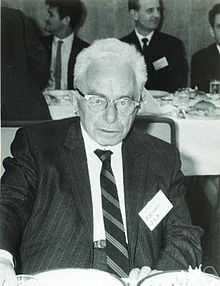
\includegraphics[height=\the\HauteurDesPhotos]{Courant}&
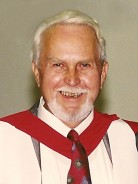
\includegraphics[height=\the\HauteurDesPhotos]{ZIENKIEWICZ}\\
Clough&Courant&Zienkiewicz%
\end{tabular}}
\medskip
\ImageADroite{%
Si on veut replacer très brièvement cela dans un contexte plus global, on peut dire que l'analyse
des structures est née vers 1850.\\
\indent
La RdM, recourant au calcul manuel,  était développée par Maxwell,\index[aut]{Maxwell (James Clerk), 1831-1879, Écossais}
Castigliano,\index[aut]{Castigliano (Carlo Alberto), 1847-1884, Italien}
Mohr.\index[aut]{Mohr (Christian Otto), 1835-1918, Allemand}\\
\indent
Le concept d'éléments finis est né vers 1940, avec des figures comme Newmark,\index[aut]{Newmark (Nathan Mortimore), 1910-1981, Américain}
Hrennikoff (1941),\index[aut]{Hrennikoff (Alexander), 1896-1984, Russe}
Mc Henry,
Courant (1942)...\index[aut]{Courant (Richard), 1888-1972, Américain}\\
\indent
Son réel essort ne commence toutefois que dans les années 60 avec le développement du
calcul numérique sur ordinateur.
}



\medskip
La méthode des éléments finis (MEF) prend ses origines dans le besoin de résoudre des problèmes
complexes d'élasticité et d'analyse de structures en ingénierie civile et aéronautique.
Son développement remonte aux travaux d'Alexander Hrennikoff (1941) et de Richard Courant (1942).
Bien qu'utilisant des approches différentes, ces deux pionniers partagent la même caractéristique
essentielle à savoir la discrétisation par maillage du domaine continu en sous-domaines discrets, que l'on
appelle éléments.
C'est Olgierd Zienkiewicz\index[aut]{Zienkiewicz (Olgierd Cecil), 1921-2009, Anglais} de l'Imperial College
qui synthétisa ces deux méthodes en ce que l'on peut appeler la méthode des éléments finis et qui fit la première formalisation
mathématique de la méthode.

\sbox{\MaBoiteAvecPhotos}{\setlength{\tabcolsep}{0pt}\scriptsize%
\begin{tabular}{ccc}%
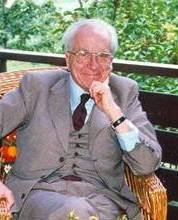
\includegraphics[height=\the\HauteurDesPhotos]{Argyris}&
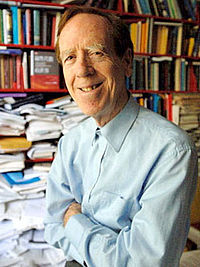
\includegraphics[height=\the\HauteurDesPhotos]{Strang}&
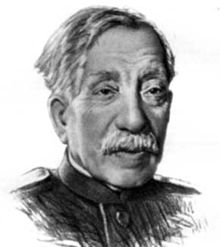
\includegraphics[height=\the\HauteurDesPhotos]{Galerkine}\\
Argyris&Strang&Galerkine%
\end{tabular}}
\medskip
\ImageAGauche{%
Dans ses travaux, Hrennikoff discrétise le domaine en utilisant une analogie avec les treillis, tandis que
l'approche de Courant divise le domaine en sous-régions finies triangulaires pour résoudre les
EDP elliptiques du second ordre issues du problème de la torsion d'un cylindre.
On peut dire que la contribution de Courant était une évolution s'appuyant sur un vaste corpus de
résultats antérieurs pour les EDP développés par Rayleigh,\index[aut]{Rayleigh (John William Strutt, troisième baron -), 1842-1919, Anglais}
Ritz\index[aut]{Ritz (Walther), 1878-1909, Suisse} et Galerkin.\index[aut]{Galerkine (Boris), 1871-1945, Russe}
}

\medskip
Le développement de la méthode des éléments finis a véritablement commencé au milieu de années 1950 pour l'analyse
structurale et aéronautique, et prit de l'ampleur à l'Université de Stuttgart grâce au travail de
John Argyris\index[aut]{Argyris (John Hadji), 1913-2004, Grec} et à Berkeley grâce au travail de
Ray W. Clough\index[aut]{Clough (Ray William), 1920-?, Américain} dans le 1960 pour l'utilisation dans
le génie civil.

\medskip
À la fin des années 50, les concepts clés de matrice de rigidité et d'assemblage d'éléments existaient
quasiment sous la forme actuelle.
La NASA publia une demande de propositions pour le développement du logiciel d'éléments finis NASTRAN en 1965.

\medskip
La base mathématique rigoureuse de la méthode des éléments finis a été consolidée en 1973 avec la publication de
Strang\index[aut]{Strang (William Gilbert), 1934-, Américain} et
Fix\index[aut]{Fix (George J.), 1939-2002, Américain} de \emph{An Analysis of The Finite Element Method}.
Elle a depuis été intégrée comme une branche des mathématiques appliquées à la modélisation
numérique des systèmes physiques dans une large variété de disciplines.
\end{histoire}
\colorblack

On veillera également à ce que les éléments ne soient pas trop
\textcolorblue{distordus}. Des critères dits <<~de forme~>> existent. Néanmoins, dans
certains cas il est possible de violer allègrement ces critères tout en
obtenant une très bonne approximation de la solution.


\medskip
Bien que la méthode des éléments finis soit théoriquement généralisable à toutes les dimensions d'espace et à
tous les ordres de dérivation, dans la pratique, l'augmentation de ces paramètres accroît de
manière dramatique la difficulté et on se contente de résoudre des problèmes limités à
\textcolorred{trois dimensions en espace et deux ordres de dérivation}.

Par exemple, un problème à trois dimensions d'espace et une dimension de temps,
qui pourrait être discrétisé par une formulation à quatre dimensions
\textcolorgris{(les éléments finis espace-temps existent)}, sera traité par
une discrétisation EF à trois dimensions d'espace couplé à un schéma en
différences finis en temps.

Pour des problèmes avec des ordres de dérivations supérieurs \textcolorgris{(des
techniques dites d'ordres élevés existent)}, comme par exemple en statique des poutres
où l'on  a une dérivation partielle d'ordre 4, on introduit des variables supplémentaires
afin de diminuer les ordres des dérivées (déformations, contraintes... \textcolorgreen{cela
a été évoqué en parlant du <<~choix des variables~>> en mécanique, nous
détaillerons un peu plus loin la formulation EF de ces formulations mixtes}).


\medskip
\section{Problèmes de la modélisation <<~réelle~>>}

Pour faire suite aux dernières remarques faites au paragraphe précédent, il faut
se rendre à l'évidence que les équations qui modélisent les principales théories
de la physique ont été présentées (et développées) dans un \textcolorred{cadre
idéalisé}.
Dans les problèmes réels, il est souvent difficile de rester dans ce cadre à cause de
nombreuses difficultés telles que les problèmes géométriques, d'échelle et du couplage
de différents modèles.

Toutefois, cela ne signifie pas qu'il est alors impossible de simuler le problème, mais seulement
qu'il est nécessaire d'ajouter encore un peu plus d'intelligence et d'astuce.
En effet, ces difficultés peuvent souvent être \textcolorblue{découplées} dans un
calcul numérique par des algorithmes adéquats et l'on se ramène alors à la
\textcolorblue{résolution itérée de problèmes standard}
(d'où la nécessité de disposer de méthodes sûres et performantes pour calculer
des solutions numériques de ces problèmes standard).

\medskip
Nous allons présenter quelques exemples de problèmes pouvant survenir
dans une modélisation, sachant qu'un certains nombre seront traités dans des
chapitres ultérieurs (mais pas tous).

\medskip
\subsection{Problèmes géométriques}
Jusqu'à présent, nous avons supposé que le domaine $\Omega$ dans lequel le problème
était considéré était fixe.
Or, dans de nombreux problèmes ce \textcolorred{domaine est variable}, on parle de
\textcolorblue{problèmes  à surface libre}, dont voici quelques exemples:
\begin{itemize}
\item Le problème le plus évident pour le lecteur, et qui a déjà été évoqué, est celui de la \textcolorblue{grande déformation} d'un solide.
\item L'étude des mouvements d'un liquide, notamment les vagues ou le mouvement de l'eau
	dans un réservoir.
	Quand la variation de la forme du domaine n'est pas trop grande on peut définir
	le domaine inconnu comme l'image d'un domaine fixe par une certaine fonction.
	Cette fonction devient alors une inconnue du problème qui se ramène à une équation
	plus complexe que l'équation initiale mais sur un domaine fixe.
	Mais, parfois, le domaine peut être amené à se fragmenter comme dans le cas de la
	formation de gouttes...
   \item La fusion de la glace dans l'eau : la frontière entre la glace et l'eau est alors une inconnue
	du problème.
\end{itemize}

\medskip
\subsection{Problèmes d'échelle}
La formulation d'un problème peut dépendre de l'échelle à laquelle on regarde
ce problème, comme cela a été mentionné précédemment.
Mais il se peut également que différentes échelles interagissent...

Quelques problèmes classiques d'échelle sont:
\begin{itemize}
   \item Nous avons déjà évoqué un peu cela en mécanique des fluides:
	dans l'écoulement d'un fluide la \textcolorblue{turbulence} est un phénomène qui fait apparaître
	des mouvements à très petite échelle. La complexité de ces mouvements rend nécessaire,
	dans un calcul numérique, le remplacement des valeurs exactes des champs inconnus par leur
	moyenne, en un sens à préciser. Cela conduit à des modèles de turbulence qui se
	différencient par les hypothèses supplémentaires qui sont faites.
   \item Dans un champ plus proche des considérations du lecteur, on pensera évidemment
	aux ondes.
	Une \textcolorblue{excitation à très haute fréquence} crée une onde de longueur très petite.
	Or une longueur d'onde très petite ne peut pas être prise en compte dans un calcul
	numérique à grande échelle. La prise en compte de ce phénomène dans l'équation
	des ondes conduit à des modèles asymptotiques dans lesquels l'étude des ondes se
	ramène à la théorie de l'optique géométrique plus ou moins enrichie pour tenir
	compte de phénomènes comme la diffraction.

	Mais si la longueur d'onde est proche des longueurs des variations géométriques
	du bord du domaine d'étude il faut revenir à l'équation des ondes pour étudier
	l'effet de ces variations géométriques. On peut donc être amener à coupler
	l'optique géométrique et une étude directe de l'équation des ondes.
   \item Un autre champ lui-aussi déjà mentionné est celui des \textcolorblue{hétérogénéités
	d'un milieu continu}, qui,  quand elles sont à très petite échelle, peuvent empêcher
	la prise en compte exacte de celles-ci, au moins dans une approximation numérique.

	C'est le cas des solides formés de matériaux composites, des fluides comme l'air
	chargé de gouttelettes d'eau ou de l'eau contenant des bulles de vapeur.
	On est conduit à définir des modèles limites dits homogénéisés
	dans lesquels on remplace les grandeurs usuelles (vitesse, masse volumique), qui ont une forte
	variation locale, par leur valeur moyenne.

	Les équations obtenues peuvent avoir la même forme que les équations initiales
	comme dans le cas de la théorie élastique des matériaux composites (le seul
	problème est de calculer les propriétés matérielles du matériau homogénéisé,
	mais nous présenterons cela plus loin) ou bien, quand les paramètres des
	hétérogénéités (la densité de bulles par exemple) dépendent de la solution,
	ces paramètres s'ajoutent aux grandeurs inconnues initiales et le nombre d'équations
	peut donc s'accroître.
\end{itemize}

\medskip
\subsection{Couplage géométrique}
De nombreux problèmes impliquent la prise en compte de plusieurs modèles selon le point
considéré.

C'est le cas de l'\textcolorblue{interaction d'un fluide et d'une structure}
(l'écoulement d'un fluide par exemple peut faire vibrer une structure qui en retour fait vibrer le fluide).
Une des difficultés vient de ce que les inconnues utilisées dans la modélisation de chacun
des milieux sont de natures différentes : les déplacements dans le solide et les vitesses dans le fluide.

Comme illustration de ce couplage, nous proposons le cas d'un poisson, issu de l'intéressante étude de
San Mart\'in et al.\index[aut]{San Mart\'in (Jorge), ?- , Chilien}
Le déplacement d'un poisson dans son millieu, illustré à la \fig{Fig-fish}.a, n'est pas imposé mais résulte
de l'interaction entre la déformation propre du poisson (donnée à la \fig{Fig-fish}.b, et qui elle est imposée)
et le fluide.
\begin{figure}[htb]
\begin{center}
  \begin{tabular}{cc}
   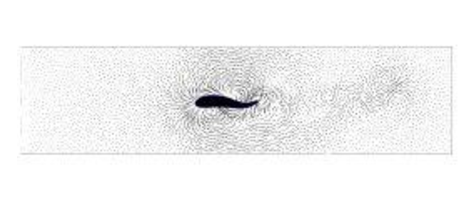
\includegraphics[height=32mm]{fish1.eps} &% ~~~
   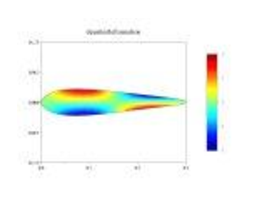
\includegraphics[height=32mm]{fish0.eps}\\
   a) poisson et son environnement & b) déformation
  \end{tabular}
\end{center}
\caption{Interaction fluide/structure: déplacement d'un poisson}
\label{Fig-fish}
\end{figure}

On retrouve aussi les problèmes d'interaction fluide/structure dans la \textcolorblue{modélisation de la circulation sanguine}:
le sang est un liquide très faiblement compressible, alors que les vaisseaux sanguins sont déformables et susceptibles
de grands déplacements

Le \textcolorblue{contact} entre deux solides peut également être placé dans cette
catégorie.


\medskip
\subsection{Couplage intrinsèque}

L'étude de la convection naturelle d'un fluide, pour la météorologie par exemple, se
modélise par le couplage des équations de la dynamique des fluides d'une part, de la
diffusion et du transport de la chaleur d'autre part: ce sont en effet les variations de
température qui créent les variations de densité responsables du mouvement de l'air,
mais ce mouvement lui-même entraîne un transport de chaleur responsable de
variations de la température. Même si l'on considère un modèle simplifié
linéarisé pour modéliser l'écoulement du fluide, le couplage fait apparaître une
non linéarité.

L'étude des plasmas oblige à coupler les équations de dynamiques des fluides et les
équations de Maxwell puisque ce sont les forces électromagnétiques qui font se mouvoir
les particules chargées mais leur mouvement est lui même la cause d'un champ
électromagnétique induit.

\medskip
\section{Principe de la méthode: résolution d'un système matriciel}

Soit $\Omega$ un domaine ouvert de $\RR^n$ ($n = 1, 2$ ou $3$ en pratique),
de frontière $\Gamma=\partial\Omega$ et sur lequel on cherche à résoudre une
EDP munie de conditions aux limites.

\medskip
Ce problème, mis sous forme variationnelle, est:
\begin{equation}\label{Eq-P}
\text{ Trouver } u\in  V \text{ tel que } a(u,v) = f(v),\quad \forall v\in V
\end{equation}
où $V$ est un espace de Hilbert.
On supposera également que l'équation de départ a de bonnes propriétés,
i.e. que l'on est dans les hypothèses vues précédemment permettant d'affirmer
que le problème admet une solution unique $u$.

\medskip
La méthode des éléments finis se propose de \textcolorblue{discrétiser} le problème considéré.
La discrétisation intervient à plusieurs niveaux:
\begin{itemize}
   \item \textcolorblue{discrétisation}:
	il est nécessaire de disposer d'une description du domaine $\Omega$ sur lequel
	on souhaite travailler. Cette description va se faire en l'approchant par
	un \textcolorblue{maillage}, qui sera constitué d'\textcolorblue{éléments}.
   \item \textcolorblue{interpolation}:
	il est ensuite nécessaire de disposer d'une manière de représenter le ou
	les champs inconnus. Ce que se proposer de faire la MEF, c'est d'approcher
	ces champs par des fonctions plus simples (disons polynomiales de
	degré un ou deux) définies sur chacun des éléments du maillage
	(le champ est approché par des bouts de fonctions qui, elles, ne sont définies
	chacune que sur un seul élément).
   \item \textcolorblue{approximation}:
	selon le type d'approximation, on remplace non seulement l'espace $V$
	(qui correspond, selon les notations utilisées au chapitre sur la formulation faible, aux espaces
	$H$, $V$, $M$ ou même $H\times M$), de dimension infinie, par des approximations $V_h$
	de dimension finie, mais parfois également les formes bilinéaires et linéaires définissant
	le problème (nous expliquerons plus tard les motivations).
\end{itemize}

\medskip
De manière classique, on notera $\mathcal{T}_h$ le maillage de $\Omega$ considéré.

Il est caractérisé par les dimensions géométriques représentatives que sont
le \textcolorblue{diamètre maximum des éléments, $h$}\index{Diamètre d'un EF}
et le \textcolorblue{facteur de forme du maillage,\index{Facteur de forme du maillage}
$\sigma$} (qui caractérise l'applatissement du maillage).

Le maillage est constitué d'éléments, généralement notés $K$.
On note $h_K$ le \textcolorblue{diamètre de l'élément $K$},\index{Diamètre d'un EF}
 i.e. le maximum des distances (euclidiennes)\index[aut]{Euclide, -325-- -265, Grec}
entre deux points de $K$, et $\rho_K$ la \textcolorblue{rondeur de l'élément $K$},\index{Rondeur d'un EF}
i.e. le diamètre maximum des sphères incluses dans $K$.
\begin{figure}[ht]
\begin{center}
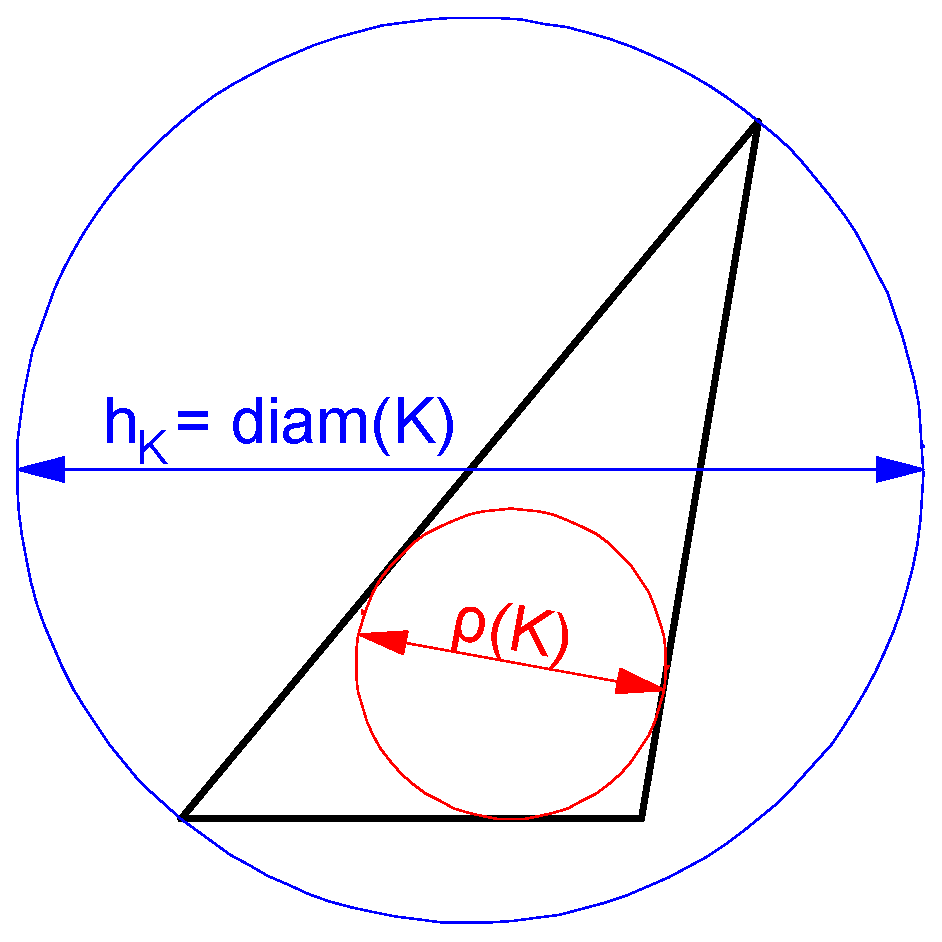
\includegraphics[width=40mm]{h-rho}
\end{center}
\caption{\label{h-rho} Dimensions géométriques caractéristiques d'un élément.}
\end{figure}

On a donc évidemment
$h_K\le h, \forall K\in\mathcal{T}_h$
puisque par définition $h=\max_{K\in\mathcal{T}_h} h_K$,
et $\frac{h_K}{\rho_K}\le\sigma, \forall K\in\mathcal{T}_h$.

On notera $\hat{K}$ l'\textcolorblue{élément de référence} correspondant à
l'élément $K$ du maillage $\mathcal{T}_h$, et d'une manière générale on ajoutera
ce <<~chapeau~>> $\hat{~}$ sur toute quantité relative à un élément de référence
(voir plus loin le chapitre sur la formulation pratique des EF).

\medskip
Les types d'approximation du problème (\ref{Eq-P}), qui seront détaillés un peu plus loin,
sont:\index{Approximation conforme}\index{Approximation non conforme}
\begin{table}[!ht]\centering\small
\begin{tabular}{cccl}
   type d'approximation & espaces & formes & problème $(P) \Rightarrow$ problème approché $(P_h)$\\
   \hline
   conforme 	  & $V_h\subset V$ & inchangées & Trouver $u_h\in V_h$ tq $a(u_h,v_h) = b(v_h), \forall v_h\in V_h$\\
   non conforme & $V_h\subset V$ & approchées & Trouver $u_h\in V_h$ tq $a_h(u_h,v_h) = b_h(v_h), \forall v_h\in V_h$\\
   non conforme & $V_h\not\subset V$ & approchées & Trouver $u_h\in V_h$ tq $a_h(u_h,v_h) = b_h(v_h), \forall v_h\in V_h$\\
   \hline
\end{tabular}
\caption{Relations approximation et espaces}
\end{table}
\textcolorgreen{En fait, on expose généralement les méthodes à partir de la méthode
dite conforme selon le tableau ci-dessus, alors qu'en pratique on travaille souvent dans le
second cas, i.e. approximation conforme en espace (i.e. $V_h\subset V$) mais non conforme
concernant les formes, car au moins les intégrations sont réalisées numériquement.}

\medskip
Toujours est-il que dans tous les cas, l'espace $V$ est remplacé par un espace $V_h$, de dimension
finie $N_h$, dont $(e_1,\ldots, e_{N_h})$ en est une base.
L'approximation $u_h$ de $u$ dans cette base s'écrit:
\begin{equation}
u_h=\dsum_{i=1}^{N_h} q_i e_i
\end{equation}
\medskip
Le problème de la méthode des éléments finis devient donc:
\begin{equation}
\text{ Trouver } q_1,\ldots, q_{N_h} \text{ tels que }
\dsum_{i=1}^{N_h} q_i a_h(e_i,v_h) = f_h(v_h) \quad , \forall v_h\in V_h
\end{equation}
soit, en exploitant les linéarités de $a_h(\cdot,\cdot)$ et $f_h(\cdot)$ et en décomposant $v_h$:
\begin{equation}\label{Eq-Ph}
\text{ Trouver } q_1,\ldots, q_{N_h} \text{ tels que }
\dsum_{i=1}^{N_h} q_i a_h(e_i,e_j) = f_h(e_j) \quad ,\forall j=1,\ldots, N_h
\end{equation}
\medskip
Il s'agit donc de résoudre le système linéaire:
\begin{equation}
\MMM{\begin{array}{ccc}
a_h(e_1,e_1) & \dots & a_h(e_{N_h},e_1)\\
$\vdots$ & & $\vdots$ \\
a_h(e_1,e_{N_h}) & \dots & a_h(e_{N_h},e_{N_h})\\
\end{array}}
\VVV{\begin{array}{c}
q_1\\
$\vdots$\\
q_{N_h}\\
\end{array}}
=
\VVV{\begin{array}{c}
f_h(e_1)\\
$\vdots$\\
f_h(e_{N_h})\\
\end{array}}
\end{equation}
que l'on note (dans la tradition mécanicienne):
\begin{equation}\mathbf{Kq=F} \quad \text{ ou encore } \quad \MMM{K}\VVV{q}=\VVV{F}
\end{equation}
\medskip
Telle que formulée, la matrice $\MM{K}$ semble pleine à priori.
L'astuce consiste à choisir des fonctions de base $e_i$ dont le support sera petit,
i.e. chaque fonction $e_i$ sera nulle partout sauf sur quelques mailles.
Ainsi les termes $a(e_i,e_j)$ seront le plus souvent nuls et la matrice A sera creuse.
De plus, on ordonnera les $e_i$ de sorte que $\MM{K}$ soit à structure bande, avec une
largeur de bande la plus faible possible.
Il existe un moyen avantageux de stocker une matrice creuse qui s'appelle le
\textcolorblue{stockage en ligne de ciel} ou \textcolorblue{skyline}.


\medskip
Les difficultés majeures en pratique sont de trouver les $e_i$ et de les manipuler
pour les calculs d'intégrales nécessaires à la construction de $\MM{K}$.
Indiquons d'ores et déjà que la plupart de ces difficultés seront levées
grâce à trois idées principales qui seront détaillées au chapitre sur
la formulation pratique des EF:
\begin{description}
 \item[Principe d'unisolvance]

	On s'attachera à trouver des \textcolorblue{degrés de liberté} (ou
	ddl) tels que la donnée de ces ddl détermine de façon univoque
	toute fonction de $V_h$.
	Il pourra s'agir par exemple des valeurs de la fonction en quelques points.
	Déterminer une fonction reviendra alors à déterminer ses valeurs sur ces ddl.
   \item[Définition des $e_i$]

	On définira les fonctions de base par $e_i = 1$ sur le $i$ème ddl, et
	$e_i = 0$ sur les autres ddl.
	La manipulation des $e_i$ sera alors simplifiée, et les $e_i$
	auront par ailleurs un support réduit à quelques mailles.

	\item[Notion de <<~famille affine d'éléments~>>]

	Le maillage sera tel que toutes les mailles soient identiques à une
	transformation affine près.
	De ce fait, tous les calculs d'intégrales pourront se ramener à
	des calculs sur une seule maille de référence, par un simple changement
	de variable.
\end{description}
\medskip
Notons que la matrice $\MM{K}$ est appelée \textcolorblue{matrice de rigidité} par
analogie avec la mécanique des solides.

\medskip
Si la forme bilinéaire $a$ est coercive, alors $\MM{K}$ est symétrique, définie positive
donc inversible. On obtient donc l'existence et l'unicité de $\VV{q} = \MMI{K}\VV{F}$.

De nombreuses méthodes permettent de résoudre le système matriciel (d'inverser la
matrice de rigidité): Gauss, mais également toutes sortes de décomposition de la matrice
de rigidité comme LU, LDLT, LLT (Cholesky).\index[aut]{Cholesky (André-Louis), 1875-1918, Français}
Lorsque $K$ est symétrique définie-positive, la méthode de Cholesky\index[aut]{Cholesky (André-Louis), 1875-1918, Français}
est la meilleure. Elle consiste à décomposer la matrice $A$ en le produit $L.L^T$,
où la matrice $L$ est une matrice triangulaire inférieure.


\medskip
\section{Approximation conforme et lemme de Céa}
\index[aut]{Cea@Céa (Jean), ?- , Français}\index{Approximation conforme}\index{Lemme de Céa}

Dans le cas d'une \textcolorblue{approximation conforme (dite aussi approximation
interne)}, on se propose de construire un espace $V_h$, de dimension $N_h$, comme
étant un \textcolorred{sous-espace vectoriel de $V$}.


\medskip
%\subsection{Principe général}
\subsection{Cas Lax-Milgram}
\index[aut]{Lax (Peter), 1926-, Américain}\index[aut]{Milgram (Arthur Norton), 1912-1961, Américain}\index[aut]{Cea@Céa (Jean), ?- , Français}\index{Théorème!de Lax-Milgram}\index{Lemme de Céa}

On se place dans la cas d'une formulation relevant du théorème de Lax-Milgram.

$V_h$ étant de dimension finie, c'est un fermé de $V$.
$V$ étant un espace de Hilbert, $V_h$ l'est donc aussi.
D'où l'existence et l'unicité de $u_h$, à partir de Lax-Milgram.

\medskip
L'espace $V_h$ sera en pratique construit à partir d'un maillage du domaine $\Omega$,
et l'indice $h$ désignera la \textcolorblue{taille typique} des mailles.
Lorsque l'on construit des maillages de plus en plus fins, la suite de sous-espaces
$(V_h)_h$ formera une \textcolorblue{approximation interne de $V$} , i.e.
pour tout élément $\varphi$ de $V$, il existe une suite de $\varphi_h\in V_h$
telle que $\|\varphi-\varphi_h\|\rightarrow 0$ quand $h\rightarrow 0$.

Cette méthode d'approximation interne est appelée \textcolorblue{méthode de
Galerkine} \textcolorgris{(Galerkine ou Galerkin)}.\index[aut]{Galerkine (Boris), 1871-1945, Russe}



\medskip
%\subsection{Signification de $u_h$}
\paragraph{Signification de $u_h$}
On a $a(u,v) = f(v)$, $\forall v\in V$, donc en particulier
$a(u,v_h) = f(v_h)$, $\forall v_h\in V_h$, car $V_h\subset V$.
Par ailleurs, $a(u_h,v_h) = f(v_h)$, $\forall v_h\in V_h$.
Par différence, il vient $a(u-u_h,v_h) = 0$, $\forall v_h\in V_h$.

Dans le cas où $a(\cdot,\cdot)$ est symétrique, il s'agit d'un produit scalaire sur $V$.
$u_h$ peut alors être interprété comme la \textcolorgreen{projection
orthogonale de $u$ sur $V_h$ au sens de $a(\cdot,\cdot)$.}


\medskip
%\subsection{Estimation d'erreur: lemme de Céa}
\begin{lemme}[Lemme de Céa]
$a(\cdot,\cdot)$ étant continue (de constante de majoration $M$) et coercitive
(de constante de minoration $\alpha$), il est aisé d'obtenir la majoration
de l'erreur appelée \textcolorblue{lemme de Céa:}
\begin{equation}
\|u-u_h\|\le\dfrac{M}{\alpha}\|u-v_h\|, \forall v_h\in V_h
\quad \text{ c'est-à-dire } \quad
\|u-u_h\|\le\dfrac{M}{\alpha}d(u,V_h)
\end{equation}
où $d$ est la distance induite par la norme $\|\cdot\|$.
\end{lemme}

Cette majoration donnée par le lemme de Céa ramène l'étude de l'\textcolorblue{erreur
d'approximation} $\|u-u_h\|$ à celle de l'\textcolorblue{erreur d'interpolation} $d(u,V_h)$.



\medskip
\subsection{Cas Babuška}
\index[aut]{Babuška (Ivo Milan), 1926-, Tchèque}\index[aut]{Cea@Céa (Jean), ?- , Français}\index{Lemme de Céa}
\index{Théorème!de Babuška}
On se place cette fois dans le cas d'un problème relevant du théorème de Babuška.
Le problème est ($v$ est dans $M$ et non plus $V$):
\begin{equation}\label{Eq-Pp}
\text{ Trouver } u\in  V \text{ tel que } a(u,v) = f(v), \forall v\in M
\end{equation}
L'approximation conforme du problème (\ref{Eq-Pp}) est le problème approché:
\begin{equation}\label{Eq-Pph}
\text{ Trouver } u_h\in V_h \text{ tel que } a(u_h,v_h) = f(v_h), \forall v_h\in M_h
\end{equation}
où $V_h\subset V$ et $M_h\subset M$.
\medskip
\textcolorred{Attention : rien ne garantit à priori que la condition inf-sup discrète
sera vérifiée, même si la condition inf-sup est vérifiée.}
$V_h$ et $M_h$ étant de dimension finie, il faut nécessairement que $\dim V_h=\dim M_h$.
\medskip
Le problème (\ref{Eq-Pph}) est bien posé, i.e. admet une unique solution, si:
\begin{equation}\left\{
\begin{aligned}
&\displaystyle\exists\alpha_h>0 \text{ tel que } \inf_{v_h\in V_h}\sup_{w_h\in M_h}\dfrac{a(v_h,w_h)}{\|v_h\|_{V_h}\|w_h\|_{M_h}}\ge\alpha_h\\
&\forall w_h\in M_h,\quad \left(a(v_h,w_h)=0\right)\Rightarrow(w_h=0)
\end{aligned}
\right.\end{equation}
ce qui est équivalent aux conditions:
\begin{equation}\left\{
\begin{aligned}
&\displaystyle\exists\alpha_h>0 \text{ tel que } \inf_{v_h\in V_h}\sup_{w_h\in M_h}\dfrac{a(v_h,w_h)}{\|v_h\|_{V_h}\|w_h\|_{M_h}}\ge\alpha_h\\
&\dim V_h=\dim M_h
\end{aligned}
\right.\end{equation}
Le première relation est appelée \textcolorblue{condition inf-sup discrète}.

\textcolorred{Attention : ces propriétés doivent être démontrées.}

\medskip
On dispose de plus de la majoration d'erreur suivante:
\begin{equation}
\|u-u_h\| \le \left(1+\dfrac{M}{\alpha_h}\right) \inf_{v_h\in V_h} \left\{\|u-v_h\|\right\}
\end{equation}
\medskip
\subsection{Cas Brezzi}
\index[aut]{Brezzi (Franco), 1945-, Italien}\index[aut]{Cea@Céa (Jean), ?- , Français}\index{Théorème!de Brezzi}\index{Lemme de Céa}
On se place cette fois dans le cas d'un problème relevant du théorème de Brezzi
(problème mixte).
Le problème est de trouver ($u, \lambda)$ dans $H\times M$ tels que:
 \begin{equation}\label{Eq-PMi}
\left\{
\begin{aligned}
 &a(u,v) + b(v, \lambda) = \langle f,v\rangle \quad \forall v\in H,\\
&b(u,\mu) = \langle g,\mu\rangle \quad \forall \mu \in M.
\end{aligned}\right.
\end{equation}
\medskip
Dans ce cas, on va faire une hypothèse forte d'injection continue...
\medskip
Le problème discrétisé correspondant à (\ref{Eq-PMi}) est bien posé, si:
le problème (\ref{Eq-PMi}) vérifie les conditions de Brezzi, et si
$(H_h\hookrightarrow H, M_h\hookrightarrow M)$ vérifie les conditions de
Brezzi (de constantes $\alpha^*$ et $\beta^*$).
\medskip
De plus, on dispose alors de la majoration d'erreur:
\begin{equation}
\|u-u_h\|_H + \|\lambda-\lambda_h\|_M \le C\left[
\inf_{v_h\in H_h} \|u-v_h\|
+ \inf_{\mu_h\in M_h} \|\lambda-\mu_h\|
\right]
\end{equation}
où la constante $C$ ne dépend que de $\|a\|$, $\alpha^*$ et
$\beta^*$.


\medskip
\section{Approximations non conformes et lemmes de Strang}
\index[aut]{Strang (William Gilbert), 1934-, Américain}\index{Approximation non conforme}\index{Lemme de Strang}

Lorsque les formes linéaires et linéaires définissant le problèmes doivent
être approchées, on se trouve alors en présence d'une \textcolorblue{approximation
non conforme}.
Comme mentionné, il existe deux types d'approximations non conformes selon que
$V_h\subset V$ ou $V_h\not\subset V$.
\medskip
\subsection{Cas $V_h\subset V$}\index[aut]{Strang (William Gilbert), 1934-, Américain}\index{Approximation non conforme}\index{Lemme de Strang}

Le problème est donc:
\begin{equation}
\text{ Trouver } u_h\in V_h \text{ tel que } a_h(u_h,v_h) = f_h(v_h), \forall v_h\in V_h
\end{equation}
où $V_h\subset V$ est de dimension finie, et $a_h$ et $f_h$ sont des approximations
de $a$ et $f$ définies sur $V_h\times V_h$ et $V_h$ resp.
\medskip
\textcolorgreen{Dans le pratique, $a_h$ et $f_h$ sont définies sur un espace plus grand que
$V_h$, mais pas sur $V$.}
\medskip
\paragraph{Motivation}
Considérons la forme:
\begin{equation}a(u,v)=\dint_\Omega (a\nabla u,\nabla v)(x)dx\end{equation}
Comme $a=a(x)$, le problème est: comment intégrer ?
On prend des formules d'intégrations, donc on ne calcule par $a(\cdot,\cdot)$,
mais $a_h(\cdot,\cdot)$ et $f_h(\cdot)$.
\medskip
Une majoration de l'erreur est donnée par le lemme 1 de Strang.

\begin{lemme}[Lemme 1 de Strang]
S'il existe $\alpha^*>0$ tel que $\forall h, a_h(v_h,v_h)\ge\alpha^*\|v_h\|^2, \forall v_h\in V_h$,
alors il existe une constante $C$ indépendante de $h$ telle que:
\begin{equation}
\|u-u_h\|\le C\left[
\inf_{v_h\in V_h} \left\{ \|u-v_h\| + \sup_{w_h\in V_h} \dfrac{|a(v_h,w_h)-a_h(v_h,w_h)|}{\|w_h\|}\right\}
+\sup_{w_h\in V_h}\left\{\dfrac{|f(w_h)-f_h(w_h)|}{\|w_h\|}\right\}
\right]
\end{equation}
Le premier terme $ \|u-v_h\|$ est appelé \textcolorblue{erreur d'approximation},
le reste \textcolorblue{erreur de consistence}.
\end{lemme}

\medskip
\subsection{Cas $V_h\not\subset V$}\index[aut]{Strang (William Gilbert), 1934-, Américain}\index{Approximation non conforme}\index{Lemme de Strang}
Le problème est encore:
\begin{equation}
\text{ Trouver } u_h\in V_h \text{ tel que } a_h(u_h,v_h) = f_h(v_h),\quad \forall v_h\in V_h
\end{equation}
mais $V_h\not\subset V$ est de dimension finie, et $a_h$ et $f_h$ sont des approximations
de $a$ et $f$ définies sur $V_h\times V_h$ et $V_h$ resp.

\medskip
\paragraph{Motivation}
Considérons le problème du Laplacien de Dirichlet.
L'espace $V$ est $H^1_0(\Omega)$.

On considère l'espace des éléments finis triangulaires engendrés par l'élément
ayant une pression constante par élément et les nœuds au centre des arêtes du
triangles. Nous notons cet espace $V_h$; alors $V_h\not\subset H^1(\Omega)$.
Nous prenons maintenant l'espace $V_{h,0}$ qui tient compte des C.L. de Dirichlet.
Si on prend:
\begin{equation}a(u,v)=\dint_\Omega \nabla u\cdot \nabla v\end{equation} alors, dans $\Omega$, il y a
des sauts et l'intégrale n'a pas de sens.
Par contre, si l'on considère:
\begin{equation} a_h(u_h,v_h)=\dsum_{K\in\mathcal{T}_h}\dint_K \nabla u_h\cdot\nabla v_h\end{equation}
l'intégrale sur chaque élément a un sens.

\medskip
Une majoration de l'erreur est donnée par le lemme 2 de Strang.
\begin{lemme}[Lemme 2 de Strang]
Si la norme $\|\cdot\|_h$ est définie sur $V_h+V$,
et s'il existe deux constantes indépendantes de $h$, $\alpha^*>0$ et $M^*>0$ tq:
$a_h(v,v)\ge\alpha^*\|v\|^2_h, \forall v\in V_h$ et
$|a_h(u,v)|\le M^*\|u\|_h\|v\|_h, \forall u\in V_h+V, \forall v\in V_h$,
alors: il existe une constante $C$ indépendante de $h$ telle que:
\begin{equation}
\|u-u_h\|\le C\left[
\inf_{v_h\in V_h} \left\{ \|u-v_h\|\right\} +
\sup_{w_h\in V_h} \left\{\dfrac{|a(u,w_h)-f_h(w_h)|}{\|w_h\|_h}\right\}
\right]
\end{equation}
Le premier terme $ \|u-v_h\|_h$ est appelé \textcolorblue{erreur d'approximation},
le second \textcolorblue{erreur de consistence}.
\end{lemme}



\medskip
\section{Convergence de la méthode des éléments finis en approximation conforme ou non lorsque $V_h\subset V$}\index{Approximation non conforme}\index{Approximation conforme}

Reprenons un cadre général, i.e. considérons $\Omega$ notre domaine
de $\RR^n$, et notre problème que nous résolvons de manière approchée
par la MEF.
Il s'agit maintenant de fournir une estimation de l'erreur $\|u-u_h\|_m$ dans $H^m$
(souvent $m = 0$, $1$ ou $2$).
La régularité de $u$ et de $u_h$ (et donc les valeurs possibles pour $m$) dépendent
du problème continu considéré ainsi que du type d'éléments finis choisis pour sa
résolution.

\medskip
On rappelle que $\mathcal{T}_h$ est le maillage de $\Omega$ considéré.
On supposera de plus le domaine $\Omega$ \textcolorred{polygonal},
ce qui permet de le recouvrir exactement par le maillage.
Si ce n'est pas le cas, il faut prendre en compte de \textcolorred{l'écart} entre le domaine couvert
par le maillage et le domaine réel.


\medskip
\subsection{Calcul de la majoration d'erreur}

Les étapes du calcul de la majoration de l'erreur sont les suivantes:
\begin{itemize}
   \item $\|u-u_h\|_m\le C\|u-\pi_hu\|_m$: l'erreur d'approximation est bornée par l'erreur
	d'interpolation;
   \item $\|u-\pi_hu\|^2_m=\dsum_{K\in\mathcal{T}_h}\|u-\pi_hu\|^2_{m,K}$:
	décomposition en majorations locales sur chaque élément;
   \item $\|u-\pi_hu\|_{m,K}\le C(K)\|\hat{u}-\hat{\pi}\hat{u}\|_{m,\hat{K}}$:
	passage à l'élément de référence;
   \item $\|\hat{u}-\hat{\pi}\hat{u}\|_{m,\hat{K}}\le \hat{C}|\hat{u}|_{k+1,\hat{K}}$:
	majoration sur l'élément de référence;
   \item $\|u-\pi_hu\|_m\le C'h^{k+1-m}|u|_{k+1}$:
	assemblage des majorations locales.
\end{itemize}

\colorgris%\scriptsize
\medskip
\subsubsection{Majoration par l'erreur d'interpolation}

En appliquant le lemme de Céa à $v_h=\pi_hu$, il vient:
\begin{equation}
\|u-u_h\|\le\dfrac{M}{\alpha}\|u-\pi_hu\|
\end{equation}

\medskip
\subsubsection{Décomposition en majorations locales sur chaque élément}

\begin{equation}
\|u-\pi_hu\|^2_m=\dsum_{K\in\mathcal{T}_h}\|u-\pi_hu\|^2_{m,K}=\dsum_{K\in\mathcal{T}_h}\dsum_{l=0}^m |u-\pi_hu|^2_{l,K}
\end{equation}
et le calcul est ramené à un calcul sur chaque élément, pour toutes les semi-normes
$\|\cdot\|_{l,K}$ pour $l=0$,\ldots, $m$.

\medskip
\subsubsection{Passage à l'élément de référence}

On se sert du théorème suivant:

\begin{theoreme}
Soit $K$ un élément quelconque de $\mathcal{T}_h$, et $\hat{K}$ l'élément de
référence. Soit $F$ la transformation affine de$\hat{K}$ vers $K$:
$F(\hat{x}) = B\hat{x} + b$, avec $B$ inversible. On a :
\begin{equation}
\forall v\in H^l(K), \quad
|\hat{v}|_{l,K} \le C(l,n) \|B\|_2^l |\det B|^{-1/2} |v|_{l,K}
\end{equation}
Ce résultat n'est rien d'autre qu'un résultat de changement de variable
dans une intégrale.
\end{theoreme}
On a même:
\begin{equation}
\forall v\in H^l(K), \quad
|\hat{v}|_{l,K} \le C(l,n) \|B^{-1}\|_2^l |\det B|^{1/2} |v|_{l,\hat{K}}
\end{equation}
\medskip
%Notons $h_K$ le \textcolorblue{diamètre de l'élément $K$}, i.e. le maximum
%des distances (euclidiennes) entre deux points de $K$, et $\rho_K$ la
%\textcolorblue{rondeur de l'élément $K$}, i.e.le diamètre maximum des
%sphères incluses dans $K$.
%
%Alors, on a:
Et avec les données géométriques de l'élément:
\begin{equation}
\|B\|\le\dfrac{h_K}{\hat{\rho}} \quad\text{ et }\quad
\|B^{-1}\|\le\dfrac{\hat{h}}{\rho_K}
\end{equation}

\medskip
\subsubsection{Majoration sur l'élément de référence}
On a le théorème suivant:

\begin{theoreme}
soient $l$ et $k$ deux entiers tels que $0\le l\le k+1$.
Si $\hat{pi}\in\mathcal{L}(H^{k+1}(\hat{K}),J^l(\hat{K}))$ laisse
$P_k(\hat{K})$ invariant, i.e.  si $\forall \hat{p}\in P_k(\hat{K}), \hat{\pi}\hat{p}=\hat{p}$,
alors:
\begin{equation}
\exists C(\hat{K},\hat{\pi}), \forall \hat{v}\in H^{k+1}(\hat{K}), |\hat{v}-\hat{\pi}\hat{v}|_{j,\hat{K}}
\le C |\hat{v}|_{k+1,\hat{K}}
\end{equation}
\end{theoreme}

\medskip
\subsubsection{Majoration sur un élément quelconque}
De ce qui précède, il vient:
\begin{equation}
|v-\pi_Kv|_{l,K}\le \hat{C}(\hat{\pi},\hat{K},l,k,n) \dfrac{h_K^{k+1}}{\rho_K^l} |v|_{k+1,K}
\end{equation}
où il faut remarquer que la constante $\hat{C}$ est indépendante de l'élément $K$.

\medskip
\subsubsection{Assemblage des majorations locales}
Il ne reste plus qu'à assembler les résultats précédents pour tous les éléments $K$
du maillage $\mathcal{T}_h$ et pour toutes les valeurs des semi-normes, i.e. pour $l=0,\ldots, m$.
%Toutefois, il faut préalablement introduire les quantités représentatives du maillage que sont
%le \textcolorblue{diamètre maximum des éléments, $h$} et le \textcolorblue{facteur
%de forme du maillage, $\sigma$} (qui caractérise l'applatissement du maillage).
%
%On a $h_K\le h, \forall K\in\mathcal{T}_h$ et $\frac{h_K}{\rho_K}\le\sigma, \forall K\in\mathcal{T}_h$.

\medskip
Par majoration et sommation sur les éléments, on obtient:
\begin{equation}
\|v-\pi_hv\|_m\le C(\mathcal{T}_h,m,k,n) h^{k+1-m} |v|_{k+1}
\end{equation}

\colorblack\normalsize
\medskip
\subsection{Majoration de l'erreur}

On obtient au final, le résultat classique de majoration d'erreur:
\begin{equation}
\|u-u_h\|_m\le C h^{k+1-m} |u|_{k+1}
\end{equation}
Quelques remarques:
\begin{itemize}
   \item On rappelle que la formule précédente a été obtenue pour domaine $\Omega$
	\textcolorred{polygonal}. Si ce n'est pas le cas, elle n'est plus valable.
	Les éléments linéaires conduisent à une erreur en $O(h)$.
	Utiliser des éléments plus raffinés (de degré 2 au lieu d'éléments linéaires) permet,
	même si la géométrie n'est également ici pas décrite de manière exacte, d'obtenir une
	erreur asymptotique en $O(h^2)$.
	\textcolorgreen{Quelque soit le degré de l'approximation, si le domaine $\Omega$ n'est pas représenté
	de manière exact, alors cela revient à une modification des conditions aux limites.}
   \item Les calculs, et plus précisément les \textcolorred{intégrations}, ont été réalisées
	\textcolorred{sans erreur}.
	Si celles-ci sont faites de manière numérique, il convient d'introduire encore un
	terme correctif supplémentaire, appelé \textcolorblue{erreur de consistance} due au remplacement des
	formes par leur approximation ($a(\cdot,\cdot)$ par $a_h(\cdot,\cdot)$, $f(\cdot)$ par $f_h(\cdot)$...). Toutefois, cette
	erreur supplémentaire peut être estimée en $O(h^k)$ selon la précision du schéma
	d'intégration utilisé.
   \item Le résultat de majoration d'erreur est souvent utilisé dans le cas $m=1$.
	Comme l'espace des polynômes $P_k(\hat{k})\subset H^1(\hat{K})$, alors si
	$\hat{\pi}$ est bien défini sur $H^{k+1}(\hat{K})$, on a:
	\begin{equation}
	\text{si } u\in H^{k+1}(\Omega), \quad \|u-u_h\|_1\le C h^k |u|_{k+1}
	\end{equation}
\end{itemize} 